\documentclass{article}
\usepackage{tikz}
\usepackage{physics}
\begin{document}
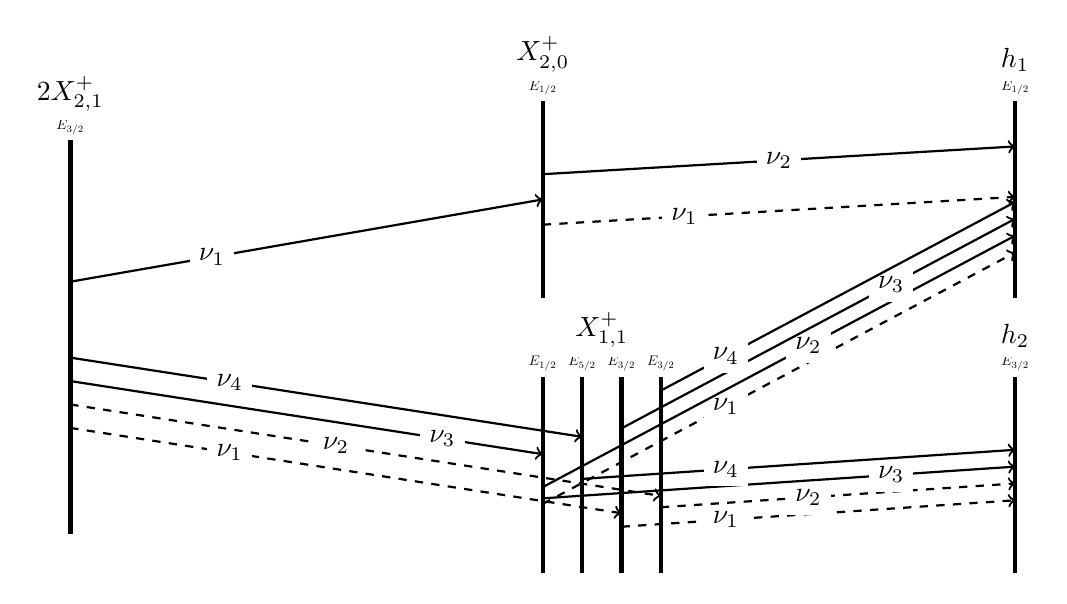
\begin{tikzpicture}[scale=0.5]
\draw[ultra thick] (-5,-1.5) -- (-5,8.5) node[above=0pt,fill=white,pos=1.0,scale=0.5] {$E_{3/2}$};
\path (-5,8.5) -- (-5,8.5) node[above=7pt,fill=white,pos=0.5,scale=1] {$2X_{2,1}^+$};
\draw[ultra thick] (7,-2.5) -- (7,2.5) node[above=0pt,fill=white,pos=1.0,scale=0.5] {$E_{1/2}$};
\draw[ultra thick] (8,-2.5) -- (8,2.5) node[above=0pt,fill=white,pos=1.0,scale=0.5] {$E_{5/2}$};
\draw[ultra thick] (9,-2.5) -- (9,2.5) node[above=0pt,fill=white,pos=1.0,scale=0.5] {$E_{3/2}$};
\draw[ultra thick] (10,-2.5) -- (10,2.5) node[above=0pt,fill=white,pos=1.0,scale=0.5] {$E_{3/2}$};
\path (7,2.5) -- (10,2.5) node[above=7pt,fill=white,pos=0.5,scale=1] {$X_{1,1}^+$};
\draw[ultra thick] (7,4.5) -- (7,9.5) node[above=0pt,fill=white,pos=1.0,scale=0.5] {$E_{1/2}$};
\path (7,9.5) -- (7,9.5) node[above=7pt,fill=white,pos=0.5,scale=1] {$X_{2,0}^+$};
\draw[ultra thick] (19,-2.5) -- (19,2.5) node[above=0pt,fill=white,pos=1.0,scale=0.5] {$E_{3/2}$};
\path (19,2.5) -- (19,2.5) node[above=7pt,fill=white,pos=0.5,scale=1] {$h_2$};
\draw[ultra thick] (19,4.5) -- (19,9.5) node[above=0pt,fill=white,pos=1.0,scale=0.5] {$E_{1/2}$};
\path (19,9.5) -- (19,9.5) node[above=7pt,fill=white,pos=0.5,scale=1] {$h_1$};
\draw[dashed,->,thick] (-5,1.19689) -- (9,-0.97026);
\path (-5,1.19689) -- (8.5,-0.89286) node[fill=white,pos=0.3] {$\nu_1$};
\draw[dashed,->,thick] (-5,1.79212) -- (10,-0.52981);
\path (-5,1.79212) -- (8.5,-0.29762) node[fill=white,pos=0.5] {$\nu_2$};
\draw[solid,->,thick] (-5,2.38736) -- (7,0.52981);
\path (-5,2.38736) -- (8.5,0.29762) node[fill=white,pos=0.7] {$\nu_3$};
\draw[solid,->,thick] (-5,2.9826) -- (8,0.97026);
\path (-5,2.9826) -- (8.5,0.89286) node[fill=white,pos=0.3] {$\nu_4$};
\draw[solid,->,thick] (-5,4.91026) -- (7,7);
\path (-5,4.91026) -- (7,7) node[fill=white,pos=0.3] {$\nu_1$};
\draw[dashed,->,thick] (9,-1.31258) -- (19,-0.64103);
\path (8.5,-1.34615) -- (19,-0.64103) node[fill=white,pos=0.3] {$\nu_1$};
\draw[dashed,->,thick] (10,-0.81807) -- (19,-0.21368);
\path (8.5,-0.9188) -- (19,-0.21368) node[fill=white,pos=0.5] {$\nu_2$};
\draw[solid,->,thick] (7,-0.59219) -- (19,0.21368);
\path (8.5,-0.49145) -- (19,0.21368) node[fill=white,pos=0.7] {$\nu_3$};
\draw[solid,->,thick] (8,-0.09768) -- (19,0.64103);
\path (8.5,-0.0641) -- (19,0.64103) node[fill=white,pos=0.3] {$\nu_4$};
\draw[dashed,->,thick] (7,-0.73443) -- (19,5.65385);
\path (8.5,0.0641) -- (19,5.65385) node[fill=white,pos=0.3] {$\nu_1$};
\draw[solid,->,thick] (7,-0.30708) -- (19,6.0812);
\path (8.5,0.49145) -- (19,6.0812) node[fill=white,pos=0.5] {$\nu_2$};
\draw[solid,->,thick] (9,1.18498) -- (19,6.50855);
\path (8.5,0.9188) -- (19,6.50855) node[fill=white,pos=0.7] {$\nu_3$};
\draw[solid,->,thick] (10,2.14469) -- (19,6.9359);
\path (8.5,1.34615) -- (19,6.9359) node[fill=white,pos=0.3] {$\nu_4$};
\draw[dashed,->,thick] (7,6.35897) -- (19,7.0641);
\path (7,6.35897) -- (19,7.0641) node[fill=white,pos=0.3] {$\nu_1$};
\draw[solid,->,thick] (7,7.64103) -- (19,8.34615);
\path (7,7.64103) -- (19,8.34615) node[fill=white,pos=0.5] {$\nu_2$};
\end{tikzpicture}
\end{document}